%%%%%%%%%%%%%%%%%%%%%%%%%%%%%%%%%%%%%%%%%%%%%%%%%%%%%%%%%%%%%%%%%%%%%%%%%%%%
%% Manuscript for Vietnam Journal of Computer Science (VJCS)
%% Class: ws-vjcs.cls (World Scientific LaTeX2e style, vjcs-2e.zip)
%% Compile: pdflatex -> bibtex -> pdflatex -> pdflatex  (or upload folder to Overleaf)
%% TODO before submission are marked with  % TODO
%%%%%%%%%%%%%%%%%%%%%%%%%%%%%%%%%%%%%%%%%%%%%%%%%%%%%%%%%%%%%%%%%%%%%%%%%%%%

\documentclass{ws-vjcs}
\usepackage{graphicx}
\usepackage[super,sort,compress]{cite}
\usepackage{url}
\usepackage{pgfplots}
\pgfplotsset{compat=1.16}

\begin{document}

\markboth{V. A. Ho}{Chunking and Segmentation for Vietnamese Legal RAG}

\catchline{0}{0}{0000}{}{}

\title{Chunking, Word Segmentation and Retrieval Strategies\\
for Vietnamese Legal RAG: An Empirical Study\\
and a Benchmark Contamination Warning}

\author{Viet Anh Ho}

\address{Faculty of Information Technology,\\
Ho Chi Minh City University of Technology and Engineering,\\
Ho Chi Minh City, Vietnam\\
hovietanh147@gmail.com}

\maketitle

\pub{Received (Day Month Year)}{Revised (Day Month Year)}

\begin{abstract}
Retrieval quality is the main bottleneck of retrieval-augmented generation (RAG) over legal text, yet how chunking, word segmentation and model choice interact for Vietnamese, whose word boundaries do not coincide with whitespace, has received little systematic study. We benchmark sparse, dense, fusion and reranking configurations on the Zalo AI 2021 legal retrieval corpus (61,425 articles), selecting configurations on 2,408 development queries and reporting on 788 test queries with paired bootstrap tests. Word segmentation improves BM25 by 2.2--2.4 nDCG@10 points in three of four chunking settings, and sentence-based chunking adds a further 3.0 points. For dense retrievers, the benefit of chunking depends on the input limit: multilingual E5 (512 tokens) gains 7.8 points, whereas BGE-M3 and EmbeddingGemma-2 (1,024 tokens) show no significant change. Reciprocal rank fusion of BM25 with three multilingual retrievers reaches 79.2 nDCG@10, 4.9 points above the best single model. Vietnamese-specific retrievers and a Vietnamese reranker score substantially higher, but one was trained on data from the same competition and the others do not disclose their training data; moreover, adding independent signals lowers their scores, the opposite of what we observe for clean models. We therefore caution against using this benchmark to rank Vietnamese retrieval models.

\keywords{Retrieval-augmented generation; Vietnamese; legal information retrieval; chunking; word segmentation; benchmark contamination.}
\end{abstract}

%=========================================================================
\section{Introduction}
%=========================================================================

Retrieval-augmented generation (RAG) grounds the output of a large language model in documents retrieved from an external collection.\cite{lewis2020rag} In the legal domain, where an unsupported answer can mislead a citizen or a practitioner, the quality of the retrieval step largely determines the quality of the final answer: if the relevant article is not retrieved, the generator cannot cite it. Building a RAG system for Vietnamese legal documents therefore starts with a set of seemingly mundane engineering decisions. How should long statutory articles be split into retrievable units? Should a lexical retriever operate on syllables or on words? Which embedding model should be used, and is it worth adding a second-stage reranker?

Vietnamese makes some of these decisions less obvious than in English. Vietnamese is written with spaces between \emph{syllables}, not words: the legal term \emph{t\`oa \'an} (``court'') consists of two space-separated syllables that form one word. A lexical retriever that tokenizes on whitespace therefore treats each syllable as an independent feature. Legal articles are also long and heterogeneous: in the corpus used here an article contains 301 syllables on average, and 10\% of articles exceed 608 syllables, which is longer than the input limit of several popular embedding models.

Practitioners often answer these questions by consulting public leaderboards. For Vietnamese legal retrieval the de facto benchmark is the Legal Text Retrieval task of the Zalo AI Challenge 2021,\cite{zalo2021legal} which is also distributed as part of the Massive Text Embedding Benchmark (MTEB).\cite{muennighoff2023mteb} During this study we found that the strongest Vietnamese-specific models on this benchmark were trained on data from the same competition, or do not disclose their training data. This raises the question of whether the benchmark still measures what practitioners need.

This paper reports a controlled empirical study organized around four research questions:
\begin{itemlist}
\item \textbf{RQ1}: Does word segmentation improve BM25 over syllable-level tokenization?
\item \textbf{RQ2}: Which chunking strategy works best for sparse and for dense retrieval?
\item \textbf{RQ3}: How do multilingual embedding models compare with Vietnamese-specific ones?
\item \textbf{RQ4}: How much do rank fusion and cross-encoder reranking add?
\end{itemlist}

A recent multi-domain benchmark compares retrieval paradigms for Vietnamese on samples of 1,000 query--passage pairs from ten datasets.\cite{nguyen2026vire} Our study is complementary: it fixes one domain and the full article collection, and varies the preprocessing decisions that such benchmarks hold constant. The main contributions of this work are summarized as follows:
\begin{itemlist}
\item We evaluate two tokenization schemes, four chunking strategies, five dense retrievers, four fusion configurations and two rerankers under identical conditions on 61,425 legal articles, selecting configurations on a separate development set and testing differences with a paired bootstrap.
\item We show that the benefit of chunking depends on the input limit of the embedding model: a 512-token model gains 7.8 nDCG@10 points, whereas 1,024-token models gain nothing significant.
\item We identify a clean and inexpensive pipeline---reciprocal rank fusion of BM25 with multilingual dense retrievers---that improves over the best single model by 4.9 points.
\item We document evidence of contamination for Vietnamese-specific models, both from model documentation and from a behavioral signal: independent retrieval signals \emph{lower} the scores of these models while they \emph{raise} the scores of clean models.
\end{itemlist}
Code and per-query results are released to support replication.

The remainder of the paper is organized as follows. Section~2 reviews related work and positions our study. Section~3 describes the data, systems and evaluation protocol. Section~4 reports results for each research question. Section~5 discusses the contamination signal, practical recommendations and limitations, and Section~6 concludes and outlines future work.

%=========================================================================
\section{Related Work}
%=========================================================================

\subsection{Vietnamese legal text retrieval}

The Zalo AI Challenge 2021 released a collection of Vietnamese legal documents segmented into articles, together with natural-language questions annotated with the articles that answer them.\cite{zalo2021legal} Subsequent work proposed multi-stage systems that combine lexical retrieval with fine-tuned neural rankers\cite{vnlegal2022multistage} and attention-based architectures for long legal documents.\cite{vnlegal2022attentive} Pre-trained Vietnamese encoders such as PhoBERT,\cite{nguyen2020phobert} which operate on word-segmented input, underlie several Vietnamese retrieval models, including the bi-encoder released by BKAI.\cite{bkai2023biencoder} The task is also part of MTEB,\cite{muennighoff2023mteb} where it is commonly used to compare embedding models on Vietnamese.

Two shared tasks have since extended this line of work. The Automated Legal Question Answering Competition (ALQAC) introduced legal document retrieval and question answering tasks for Vietnamese,\cite{nguyen2021alqac} and the DRILL shared task at VLSP 2025 asked participants to retrieve supporting articles for more than 3,000 citizen questions from a collection of about 60,000 articles; most participating systems followed a retrieve-then-rerank design that combines BM25, dense retrievers and cross-encoders.\cite{vuong2025drill} Other recent work improves Vietnamese legal retrieval by pre-training retrievers on queries generated by large language models\cite{pham2024synthetic} or by combining keyword and vector search with rank fusion in a question-answering system.\cite{ba2024legalqa} These studies mostly aim to build the strongest system; the effect of individual preprocessing choices is rarely isolated.

\subsection{Dense retrieval and reranking}

Dense retrievers encode queries and passages independently into vectors and rank passages by similarity.\cite{karpukhin2020dpr,reimers2019sbert} Late-interaction models such as ColBERT keep one vector per token and trade index size for effectiveness,\cite{khattab2020colbert} and zero-shot evaluations across many collections have shown that BM25 remains a robust baseline against which neural retrievers should be compared.\cite{thakur2021beir} Multilingual models such as multilingual E5\cite{wang2024me5} and BGE-M3\cite{chen2024bgem3} support Vietnamese without language-specific training, and recent compact models such as EmbeddingGemma\cite{vera2025embeddinggemma,gemma2emb} target on-device retrieval. Cross-encoder rerankers, which jointly encode a query and a candidate passage, typically improve the top of a ranking at a much higher computational cost.\cite{nogueira2019passage} Reciprocal rank fusion (RRF) combines rankings from heterogeneous retrievers without score calibration and remains a strong, simple baseline.\cite{cormack2009rrf}

\subsection{Retrieval granularity}

Long documents exceed the input limit of most neural encoders. A common strategy is to split documents into passages and score a document by its best passage (MaxP).\cite{dai2019maxp} The choice of retrieval unit---documents, passages, sentences or propositions---has a measurable effect on dense retrieval quality.\cite{chen2024densex} To our knowledge, the interaction between chunking and segmentation has not been studied for Vietnamese legal text.

\subsection{Benchmark contamination}

When evaluation data, or data from the same source, is included in training, benchmark scores overestimate generalization.\cite{magar2022contamination,sainz2023contamination} This concern has been raised mostly for large language models; it applies equally to embedding models and rerankers that are fine-tuned on public retrieval datasets.

\subsection{Summary and positioning}

Prior work on Vietnamese legal retrieval has largely focused on building the best system for a given competition. The recent multi-domain benchmark of Nguyen and Quan\cite{nguyen2026vire} compares lexical, sparse, late-interaction, dense and hybrid retrievers across six domains, including a ZaloLegalQA set drawn from the same competition data as ours. To make domains comparable, it evaluates each dataset on 1,000 query--passage pairs, so the candidate pool is much smaller than the full article collection; it keeps preprocessing fixed, and it reports Vietnamese\_Embedding\_v2 as the strongest dense model on ZaloLegalQA without discussing the overlap between that model's training data and the benchmark. Neither line of work isolates how word segmentation and chunking interact with the input limit of the embedding model, selects configurations on held-out data and compares them with paired per-query significance tests, or checks whether the models being ranked have seen data from the benchmark source. Our study addresses these three points on a single, full-size legal collection; it does not propose a new model.

%=========================================================================
\section{Experimental Setup}
%=========================================================================

\subsection{Data and splits}

We use the Hugging Face mirror of the Zalo AI 2021 Legal Text Retrieval data (\texttt{GreenNode/zalo-ai-legal-text-retrieval-vn}), which is also the source of the MTEB task. The corpus contains 61,425 articles; statistics are given in Table~\ref{tab:data}. The query file contains 3,196 questions with text. We use the 788 queries of the official test qrels (793 relevant query--article pairs, 1.006 relevant articles per query on average) for reporting only. The 2,408 queries of the training qrels that do not overlap with the test set form a development set, which we use for every model-selection decision: the chunking strategy of each retriever, the retrievers entering fusion, and the first stage for reranking.

\begin{table}[t]
\tbl{Corpus statistics and chunking strategies. Lengths are counted in whitespace-separated syllables.\label{tab:data}}
{\begin{tabular}{@{}lr@{}} \toprule
Statistic & Value \\ \colrule
Articles & 61,425 \\
Article length: mean / median & 301 / 197 \\
Article length: 90th percentile / max & 608 / 55,386 \\
Test queries (relevant pairs) & 788 (793) \\
Development queries & 2,408 \\ \colrule
Chunks: \texttt{article} (whole article) & 61,425 \\
Chunks: \texttt{fixed128} (128-syllable window, 25\% overlap) & 204,484 \\
Chunks: \texttt{fixed256} (256-syllable window, 25\% overlap) & 113,751 \\
Chunks: \texttt{sent256} (sentences packed up to 256 syllables) & 107,052 \\ \botrule
\end{tabular}}
\end{table}

\subsection{Chunking}

We compare four strategies (Table~\ref{tab:data}). \texttt{article} keeps each article as a single unit. \texttt{fixed128} and \texttt{fixed256} slide a window of 128 or 256 syllables with a stride of 75\% of the window. \texttt{sent256} splits an article at sentence boundaries (periods, semicolons, colons, question and exclamation marks, and line breaks) and greedily packs consecutive sentences into chunks of at most 256 syllables. Retrieval always operates on chunks, and an article receives the score of its best chunk (MaxP):\cite{dai2019maxp}
\begin{equation}
s(q, d) = \max_{c \in C(d)} s(q, c)\,,
\label{eq:maxp}
\end{equation}
where $C(d)$ is the set of chunks of article $d$. All evaluation is at the article level.

\subsection{Sparse retrieval and word segmentation}

We use Okapi BM25\cite{robertson2009bm25} with $k_1 = 1.2$, $b = 0.75$ and the Lucene variant of inverse document frequency,
\begin{equation}
\mathrm{idf}(t) = \ln\!\left(1 + \frac{N - n_t + 0.5}{n_t + 0.5}\right),
\label{eq:idf}
\end{equation}
where $N$ is the number of chunks and $n_t$ the number of chunks containing term $t$. We compare two tokenizations: \emph{syllable}, which lowercases the text and keeps alphanumeric tokens, and \emph{word}, which first applies the pyvi word segmenter\cite{pyvi} (a lightweight alternative to the VnCoreNLP toolkit\cite{vu2018vncorenlp}) so that multi-syllable words become single tokens (e.g.~\emph{t\`oa\_\'an}). The same tokenizer is applied to queries and chunks. BM25 is implemented with sparse matrices so that all queries can be scored against more than 200,000 chunks in about one minute on a CPU.

\subsection{Dense retrievers}

Table~\ref{tab:models} lists the dense retrievers. We group them by the evidence available about their training data. The \emph{clean} group consists of multilingual models with no indication of training on the Zalo legal data: multilingual E5 large,\cite{wang2024me5} BGE-M3\cite{chen2024bgem3} and EmbeddingGemma-2.\cite{gemma2emb} The \emph{Vietnamese} group consists of two models trained specifically for Vietnamese retrieval. According to its model card, the BKAI bi-encoder was trained on translated MS MARCO, translated SQuAD v2 and 80\% of the Zalo 2021 legal training set.\cite{bkai2023biencoder} The AITeamVN model card describes training on about 300,000 Vietnamese triplets without naming the sources, and states that the model was not trained on the Zalo legal data.\cite{aiteam2025embedding} We report both but draw no conclusion about Vietnamese-specific models from them (Section~\ref{sec:rq3}). We also planned to evaluate EmbeddingGemma-300m,\cite{vera2025embeddinggemma} but its gated repository was not accessible from our environment.

\begin{table}[t]
\tbl{Dense retrievers. ``Max'' is the maximum input length in tokens used in our runs.\label{tab:models}}
{\begin{tabular}{@{}llrl@{}} \toprule
Name & Hugging Face model & Max & Group \\ \colrule
e5-large & intfloat/multilingual-e5-large & 512 & clean \\
bge-m3 & BAAI/bge-m3 & 1,024 & clean \\
gemma-2 & google/embeddinggemma-2 & 1,024 & clean \\
bkai-vi & bkai-foundation-models/vietnamese-bi-encoder & 256 & Vietnamese$^\dagger$ \\
aiteam-vi & AITeamVN/Vietnamese\_Embedding & 1,024 & Vietnamese$^\ddagger$ \\ \botrule
\end{tabular}}
\begin{tabnote}
$^\dagger$Trained on 80\% of the Zalo 2021 legal training set. $^\ddagger$Training data not disclosed.
\end{tabnote}
\end{table}

All models are run with the Sentence-Transformers library,\cite{reimers2019sbert} with L2-normalized embeddings and cosine similarity. We follow each model's documented input format: the \texttt{query:}/\texttt{passage:} prefixes for E5, the \texttt{SearchQuery}/\texttt{Document} prompts for EmbeddingGemma-2 (in bfloat16, as recommended), and pyvi word segmentation for the PhoBERT-based BKAI model.

\subsection{Fusion and reranking}

Reciprocal rank fusion\cite{cormack2009rrf} scores an article $d$ by
\begin{equation}
\mathrm{RRF}(d) = \sum_{r \in R} \frac{1}{k + \mathrm{rank}_r(d)}\,,
\label{eq:rrf}
\end{equation}
with $k = 60$, where $R$ is the set of runs being fused and each run contributes its top 100 articles. Following the development-set protocol, we fuse the best BM25 configuration with one, two or all three clean dense retrievers, each in its development-selected chunking. The fused run with the highest development Recall@20 is used as the first stage for reranking, since a reranker can only promote articles that the first stage retrieves. The top 50 articles are rescored by two cross-encoders with inputs truncated to 1,024 tokens: the multilingual \texttt{BAAI/bge-reranker-v2-m3}\cite{chen2024bgem3} and \texttt{AITeamVN/Vietnamese\_Reranker}, whose model card describes training on about 1.1 million triplets without naming the sources.\cite{aiteam2025embedding} Because no selection is made after reranking, rerankers are run on the test queries only.

\subsection{Evaluation and significance testing}

We report Recall@$k$ for $k \in \{1, 5, 10, 20\}$, mean reciprocal rank at 10 (MRR@10) and nDCG@10\cite{jarvelin2002ndcg} at the article level, as percentages. Differences between two systems are tested with a paired bootstrap over test queries\cite{efron1993bootstrap,sakai2006bootstrap,smucker2007significance} with $B = 10{,}000$ resamples; we report the mean difference, the 95\% percentile confidence interval and a two-sided $p$-value. With $B = 10{,}000$, $p < 0.001$ indicates that no resample changed the sign of the difference.

\subsection{Implementation}

All experiments ran on a single NVIDIA A100 80\,GB GPU with 12 virtual CPUs (Google Colab). We ran the full pipeline twice: an exploratory run and the final run with the development-set protocol. Test scores of the configurations shared by both runs differed by at most 0.05 points, which indicates that the results are reproducible. Unless stated otherwise, numbers come from the final run; the scores of the two Vietnamese models and the pipeline built on BKAI come from the exploratory run (Section~\ref{sec:contam}).

%=========================================================================
\section{Results}
%=========================================================================

\subsection{RQ1: word segmentation for BM25}

Table~\ref{tab:bm25} reports BM25 with both tokenizations and all four chunking strategies, and Table~\ref{tab:boot} gives the corresponding significance tests. Word segmentation improves nDCG@10 in every setting, by 2.35, 1.11, 2.22 and 2.15 points; the improvement is significant for \texttt{article}, \texttt{fixed256} and \texttt{sent256} ($p \le 0.004$) but not for \texttt{fixed128} ($p = 0.125$). The gain is concentrated at the top of the ranking: in the three chunked settings, Recall@1 improves by 2.7 to 3.6 points, significantly in each case. Merging syllables into words removes spurious matches in which a query syllable such as \emph{t\`oa} matches a chunk that never mentions the word \emph{t\`oa \'an}. The additional cost is modest: a complete BM25 run with word segmentation (segmenting the corpus with 12 processes, indexing, and scoring 3,196 queries) took 66--91\,s, against 26--43\,s with syllable tokenization, and the segmentation of the corpus is needed only once.

\begin{table}[t]
\tbl{BM25 on the 788 test queries (\%). Best value per column in bold.\label{tab:bm25}}
{\begin{tabular}{@{}llrrrrr@{}} \toprule
Chunking & Tokens & R@1 & R@10 & R@20 & MRR@10 & nDCG@10 \\ \colrule
article & syllable & 44.16 & 82.49 & 86.99 & 57.63 & 63.68 \\
article & word & 46.32 & 85.98 & 91.12 & 59.68 & 66.03 \\
fixed128 & syllable & 48.29 & 84.45 & 90.04 & 61.94 & 67.47 \\
fixed128 & word & 51.02 & 85.15 & \textbf{92.70} & 63.27 & 68.58 \\
fixed256 & syllable & 47.59 & 83.57 & 88.32 & 60.93 & 66.46 \\
fixed256 & word & 50.25 & \textbf{86.42} & 91.81 & 63.04 & 68.69 \\
sent256 & syllable & 49.11 & 83.31 & 89.02 & 61.56 & 66.85 \\
sent256 & word & \textbf{52.66} & 84.96 & 91.31 & \textbf{63.90} & \textbf{69.00} \\ \botrule
\end{tabular}}
\end{table}

\subsection{RQ2: chunking}

For BM25, all three chunked strategies outperform whole articles. The development set selects \texttt{sent256} with word segmentation, which is also the best configuration on the test set and improves over whole articles by 2.97 nDCG@10 and 6.35 Recall@1 points ($p < 0.001$).

For dense retrievers the picture is different (Table~\ref{tab:dense}, Fig.~\ref{fig:chunk}). Multilingual E5, whose input is truncated at 512 tokens, benefits most: its development-selected \texttt{fixed128} configuration improves over whole articles by 7.80 points ($p < 0.001$). For the two clean models with a 1,024-token input, chunking brings no significant change: $+1.50$ points for BGE-M3 ($p = 0.121$) and $-0.69$ points for EmbeddingGemma-2 ($p = 0.427$), whose best test score is in fact obtained on whole articles. The Vietnamese models follow the same pattern: BKAI (256 tokens) gains 4.55 points from chunking, whereas AITeamVN (1,024 tokens) is best on whole articles and loses 3.85 points with \texttt{fixed128}. Chunking therefore acts mainly as a remedy for truncation. When the encoder can read most of an article, splitting it removes context and does not help; the smallest chunks are the most harmful for 1,024-token models.

\begin{table}[t]
\tbl{Dense retrieval: nDCG@10 (\%) on the test set, with the development score in parentheses for clean models. Development-selected chunking marked with $^*$.\label{tab:dense}}
{\begin{tabular}{@{}lllll@{}} \toprule
Model & article & fixed128 & fixed256 & sent256 \\ \colrule
e5-large & 66.53 (71.76) & 74.33 (77.65)$^*$ & 75.14 (77.21) & 75.39 (77.45) \\
bge-m3 & 72.14 (72.70) & 73.64 (76.69)$^*$ & 73.57 (75.94) & 72.98 (75.75) \\
gemma-2 & 71.80 (69.84) & 68.68 (71.33) & 71.10 (72.43)$^*$ & 70.85 (71.17) \\ \colrule
bkai-vi$^\dagger$ & 84.08 & 87.75 & 88.55 & 88.63 \\
aiteam-vi$^\ddagger$ & 85.39 & 81.54 & 84.33 & 84.58 \\ \botrule
\end{tabular}}
\begin{tabnote}
$^\dagger$Trained on data from the same competition. $^\ddagger$Training data not disclosed. Both from the exploratory run, without development-set selection.
\end{tabnote}
\end{table}

\begin{figure}[t]
\centering
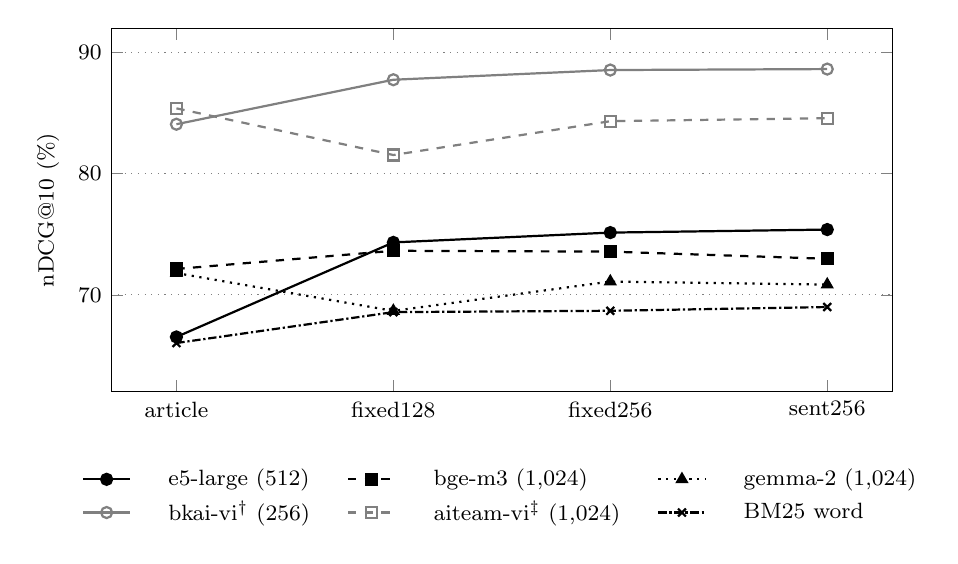
\begin{tikzpicture}
\begin{axis}[
  width=11.5cm, height=6.2cm,
  symbolic x coords={article,fixed128,fixed256,sent256},
  xtick=data,
  ylabel={nDCG@10 (\%)},
  ymin=62, ymax=92,
  ymajorgrids, grid style={dotted,gray},
  tick label style={font=\footnotesize},
  label style={font=\footnotesize},
  legend style={font=\footnotesize, at={(0.5,-0.18)}, anchor=north, legend columns=3, draw=none,
    /tikz/every even column/.append style={column sep=4mm},
    /tikz/every odd column/.append style={column sep=4mm}},
  legend cell align=left,
  every axis plot/.append style={thick, mark size=2pt, mark options={solid}}]
\addplot[black, mark=*] coordinates {(article,66.53) (fixed128,74.33) (fixed256,75.14) (sent256,75.39)};
\addplot[black, dashed, mark=square*] coordinates {(article,72.14) (fixed128,73.64) (fixed256,73.57) (sent256,72.98)};
\addplot[black, dotted, mark=triangle*] coordinates {(article,71.80) (fixed128,68.68) (fixed256,71.10) (sent256,70.85)};
\addplot[gray, mark=o] coordinates {(article,84.08) (fixed128,87.75) (fixed256,88.55) (sent256,88.63)};
\addplot[gray, dashed, mark=square] coordinates {(article,85.39) (fixed128,81.54) (fixed256,84.33) (sent256,84.58)};
\addplot[black, densely dashdotted, mark=x] coordinates {(article,66.03) (fixed128,68.58) (fixed256,68.69) (sent256,69.00)};
\legend{{e5-large (512)}, {bge-m3 (1{,}024)}, {gemma-2 (1{,}024)}, {bkai-vi$^\dagger$ (256)}, {aiteam-vi$^\ddagger$ (1{,}024)}, {BM25 word}}
\end{axis}
\end{tikzpicture}
\vspace*{4pt}
\caption{Test nDCG@10 by chunking strategy. The maximum input length of each dense model is given in parentheses. Gray lines: Vietnamese-specific models with known or possible exposure to the benchmark source.}
\label{fig:chunk}
\end{figure}

\subsection{RQ3: multilingual versus Vietnamese-specific models}
\label{sec:rq3}

Among clean models, the development set ranks e5-large first, BGE-M3 second and EmbeddingGemma-2 third, and the test scores of the selected configurations follow the same order (74.33, 73.64 and 71.10). EmbeddingGemma-2, the most recent model in our study, trails the other two by 2.5--3.2 points on this task and was about twice as slow to encode the corpus (256--421\,s against 120--199\,s on the A100). We used its documented default document prompt, which sets the title field to ``none''; supplying article titles may help and is left for future work.

The two Vietnamese-specific models score 10 to 13 points higher than the best clean model (88.63 and 85.39 against 75.39). We do not interpret this gap as evidence that Vietnamese-specific training is superior. The BKAI model was trained on 80\% of the training data of the same competition from which the test set is derived, so we cannot rule out overlap between its training data and our test queries; the AITeamVN model does not disclose its training data. Section~\ref{sec:contam} presents a behavioral signal that supports this caution.

\subsection{RQ4: fusion and reranking}

Table~\ref{tab:pipeline} reports the clean pipeline and Table~\ref{tab:boot} the significance tests. The best single dense model (e5-large, \texttt{fixed128}) outperforms the best BM25 configuration by 5.33 points ($p < 0.001$). Fusion helps consistently: adding BM25 to e5-large improves nDCG@10 by 2.89 points and Recall@1 by 5.14 points, fusing the two strongest dense models adds 1.40 points, and fusing BM25 with all three clean dense models reaches 79.19 nDCG@10, 4.86 points above e5-large alone ($p < 0.001$). The fusion step itself takes less than one second for all queries; its cost is that of running the component retrievers.

\begin{table}[t]
\tbl{Clean pipeline on the test set (\%). Configurations selected on the development set. Time is the wall-clock time of the step on the A100 for all queries.\label{tab:pipeline}}
{\begin{tabular}{@{}lrrrrrr@{}} \toprule
System & R@1 & R@10 & R@20 & MRR@10 & nDCG@10 & Time (s) \\ \colrule
BM25 (word, sent256) & 52.66 & 84.96 & 91.31 & 63.90 & 69.00 & 69 \\
e5-large (fixed128) & 55.46 & 92.51 & 96.32 & 68.59 & 74.33 & 199 \\
RRF(e5 + bge-m3) & 56.85 & 93.65 & 96.32 & 70.04 & 75.73 & $<$1 \\
RRF(BM25 + e5) & 60.60 & 93.78 & 96.57 & 71.97 & 77.21 & $<$1 \\
RRF(BM25 + e5 + bge-m3) & 59.77 & 94.29 & 96.83 & 72.29 & 77.61 & $<$1 \\
RRF(BM25 + 3 dense) & 62.31 & \textbf{94.67} & 96.83 & 74.22 & \textbf{79.19} & $<$1 \\
\quad + bge-reranker-v2-m3 & \textbf{65.74} & 94.04 & \textbf{96.95} & \textbf{76.34} & 80.61 & 268 \\ \colrule
\quad + Vietnamese\_Reranker$^\ddagger$ & 79.89 & 97.08 & 97.84 & 87.00 & 89.49 & 265 \\ \botrule
\end{tabular}}
\begin{tabnote}
$^\ddagger$Training data not disclosed; reported separately and excluded from the bold marks.
\end{tabnote}
\end{table}

Reranking the fused run with the multilingual \texttt{bge-reranker-v2-m3} raises Recall@1 by 3.43 points ($p = 0.042$) but the 1.42-point nDCG@10 gain is not significant ($p = 0.157$), for about 4.5 minutes of GPU time on 788 queries. The Vietnamese reranker adds 10.30 points of nDCG@10 and 17.58 points of Recall@1 ($p < 0.001$). As with the Vietnamese embedding models, its training data is not disclosed, and its score is close to that of the BKAI pipeline; we therefore do not include it in our recommendations.

\begin{table}[t]
\tbl{Paired bootstrap tests on the test set ($n = 788$, $B = 10{,}000$). $\Delta$ is A minus B in percentage points; CI is the 95\% interval for $\Delta$nDCG@10.\label{tab:boot}}
{\begin{tabular}{@{}lrlrrr@{}} \toprule
Comparison (A $-$ B) & $\Delta$nDCG & CI & $p$ & $\Delta$R@1 & $p$ \\ \colrule
\multicolumn{6}{@{}l}{\emph{RQ1: BM25 word $-$ syllable}} \\
\quad article & 2.35 & [0.80, 3.92] & .002 & 2.16 & .129 \\
\quad fixed128 & 1.11 & [$-$0.33, 2.55] & .125 & 2.73 & .024 \\
\quad fixed256 & 2.22 & [0.74, 3.71] & .004 & 2.66 & .049 \\
\quad sent256 & 2.15 & [0.68, 3.58] & .004 & 3.55 & .007 \\
\multicolumn{6}{@{}l}{\emph{RQ2: selected chunking $-$ article}} \\
\quad BM25 word (sent256) & 2.97 & [1.38, 4.57] & $<$.001 & 6.35 & $<$.001 \\
\quad e5-large (fixed128) & 7.80 & [5.67, 9.92] & $<$.001 & 6.47 & $<$.001 \\
\quad bge-m3 (fixed128) & 1.50 & [$-$0.39, 3.38] & .121 & 1.27 & .442 \\
\quad gemma-2 (fixed256) & $-$0.69 & [$-$2.34, 0.96] & .427 & $-$2.41 & .119 \\
\multicolumn{6}{@{}l}{\emph{RQ4: fusion and reranking}} \\
\quad e5-large $-$ BM25 & 5.33 & [3.03, 7.74] & $<$.001 & 2.79 & .153 \\
\quad RRF(BM25+e5) $-$ e5 & 2.89 & [1.18, 4.53] & $<$.001 & 5.14 & .003 \\
\quad RRF(e5+bge) $-$ e5 & 1.40 & [0.37, 2.42] & .007 & 1.40 & .186 \\
\quad RRF(BM25+e5+bge) $-$ e5 & 3.28 & [1.85, 4.71] & $<$.001 & 4.31 & .002 \\
\quad RRF(BM25+3 dense) $-$ e5 & 4.86 & [3.26, 6.40] & $<$.001 & 6.85 & $<$.001 \\
\quad + bge-reranker $-$ RRF & 1.42 & [$-$0.53, 3.41] & .157 & 3.43 & .042 \\
\quad + Vietnamese\_Reranker $-$ RRF & 10.30 & [8.36, 12.30] & $<$.001 & 17.58 & $<$.001 \\ \botrule
\end{tabular}}
\end{table}

%=========================================================================
\section{Discussion}
%=========================================================================

\subsection{A behavioral contamination signal}
\label{sec:contam}

In the exploratory run, configurations were chosen by test score, and both selected dense runs happened to be BKAI runs (\texttt{sent256}, 88.63 nDCG@10, and \texttt{fixed256}, 88.55). Table~\ref{tab:sign} contrasts the effect of the same two operations on this pipeline and on the clean pipeline. Adding BM25 through RRF improves the clean pipeline by 2.89 points but lowers the BKAI pipeline by 4.00 points. Reranking with the multilingual \texttt{bge-reranker-v2-m3} improves the clean pipeline by 1.42 points but lowers the BKAI pipeline by 6.29 points, to 82.34.

\begin{table}[t]
\tbl{Change in nDCG@10 (points) caused by the same operation on the clean pipeline and on a pipeline built on bkai-vi.\label{tab:sign}}
{\begin{tabular}{@{}lrr@{}} \toprule
Operation & Clean pipeline & bkai-vi pipeline \\ \colrule
Add BM25 via RRF & $+$2.89 & $-$4.00 \\
Rerank with bge-reranker-v2-m3 & $+$1.42 & $-$6.29 \\ \botrule
\end{tabular}}
\end{table}

Both BM25 and the multilingual reranker are independent of the Zalo legal data. For a retriever whose quality generalizes, an independent and reasonably strong signal should rarely hurt; this is what we observe for the clean models. For a retriever that has seen data from the same source as the test queries, independent signals pull the ranking toward their own, lower level of about 80 nDCG@10. The reversal of sign is not proof of contamination, but together with the model documentation it indicates that scores of Vietnamese-specific models on this benchmark should not be read as estimates of their quality on unseen legal questions. Because the MTEB version of the task uses the same data, the same caution applies to MTEB rankings on this task, and to other benchmarks that include questions from the same competition, such as the ZaloLegalQA subset of the multi-domain benchmark of Nguyen and Quan.\cite{nguyen2026vire} A clean benchmark---for example questions about legal documents issued after the release of the models under evaluation---would be needed for a fair comparison.

\subsection{Practical recommendations}

For practitioners building Vietnamese legal RAG systems, our results suggest the following:
\begin{alphlist}[(a)]
\item Segment words before indexing with BM25; the cost is incurred once and the gain is significant in most settings.
\item Chunk articles at sentence boundaries (about 256 syllables) for BM25 and for embedding models with an input limit of 512 tokens or less; for models that accept 1,024 tokens, keep whole articles or use large chunks.
\item Use RRF of BM25 with several multilingual dense retrievers as a default first stage; it gave the largest significant improvement in our study at negligible additional cost.
\item Validate a reranker on in-domain development data before deployment; a general multilingual reranker improved Recall@1 but not nDCG@10.
\item Check the documented training data of a model before relying on its benchmark scores.
\end{alphlist}

\subsection{Limitations}

Our study has several limitations. It uses one dataset and one domain and evaluates retrieval only, not the answers generated from retrieved articles. Each query has about one relevant article, so Recall@$k$ is close to a hit rate, and unlabeled relevant articles may exist. The development set is drawn from the competition's training data, which the BKAI model has partly seen; it is therefore suitable for selecting among clean models only. EmbeddingGemma-300m could not be evaluated, and EmbeddingGemma-2 was used with its default document prompt. Chunk lengths are counted in syllables rather than in model tokens. We fuse rankings with RRF because it needs no tuning; Nguyen and Quan\cite{nguyen2026vire} found linear interpolation of BM25 and dense scores to be stronger than RRF on Vietnamese data, so our fusion gains may underestimate what a tuned hybrid achieves. Finally, the bootstrap tests are not corrected for multiple comparisons; the main conclusions rest on differences with $p < 0.001$, which remain significant under a Holm--Bonferroni correction over the 15 comparisons per metric, since the strictest Holm threshold is $0.05/15 \approx 0.0033$.

%=========================================================================
\section{Conclusion and Future Work}
%=========================================================================

We studied the design space of retrieval for Vietnamese legal RAG under a development-set protocol with significance testing. Two inexpensive choices, word segmentation and chunking, improve retrieval significantly, but the benefit of chunking for dense retrievers depends on their input limit: it is large for a 512-token model and absent for 1,024-token models. Fusing BM25 with several multilingual dense retrievers is the best clean configuration we found, reaching 79.2 nDCG@10. Vietnamese-specific retrievers and rerankers score considerably higher on the standard benchmark, but their documented training data and the reversed effect of independent signals indicate that this benchmark can no longer rank such models reliably.

Several directions remain open. First, a contamination-free evaluation set, for example questions about legal documents issued after the release of the models under evaluation, is needed to compare Vietnamese-specific and multilingual models fairly. Second, the protocol should be repeated on the ALQAC and DRILL collections to test whether our findings on segmentation and chunking transfer to other legal datasets. Third, chunk lengths should be measured in model tokens rather than syllables, and smaller models such as EmbeddingGemma-300m should be included. Finally, the study should be extended from retrieval to the quality and faithfulness of answers generated in an end-to-end RAG system.

\section*{Acknowledgments}

% TODO: tai tro, cam on (neu co)
[To be completed by the authors.]

\section*{Declaration of Generative AI Use}

% TODO: tac gia doc lai va chinh sua cho dung voi thuc te
During the preparation of this work the author used Claude (Anthropic) to assist with writing experiment code, running the experiments on Google Colab and drafting the manuscript text. After using this tool, the author reviewed and edited the content as needed and take full responsibility for the content of the publication.

\section*{Data and Code Availability}

% TODO: chuyen repo GitHub sang Public truoc khi nop (link duoi day chi mo duoc khi repo da Public)
The Zalo AI 2021 legal retrieval data are publicly available as a Hugging Face dataset:
\begin{center}\texttt{GreenNode/zalo-ai-legal-text-retrieval-vn}\end{center}
Code, configuration files and per-query results are available at
\begin{center}\url{https://github.com/AndyAnh174/vietnamese-legal-rag-retrieval}\end{center}

\section*{ORCID}

\noindent Viet Anh Ho \quad \url{https://orcid.org/0009-0005-0099-2550}

\bibliographystyle{ws-vjcs}
\bibliography{refs}

\end{document}
